\documentclass[]{article}
\usepackage{amsmath}
\usepackage{amsfonts}
\usepackage{amssymb}
\usepackage{graphicx}
%opening
\title{Actor Critic Agent}
\author{Marco Marini}

\begin{document}

\maketitle

\begin{abstract}

\end{abstract}

\section{TD Error}

The TD error is defined as
\begin{equation}
\delta_t = r_t - r_\pi + v_\pi(s_{t+1}) - v_\pi(s_t)	
\end{equation}

\section{Policy actor}

The policy actor estimate the probabilities $ \pi_a(s) $ of choose action $ a $ at status $ s $.
The function is the softmax of the actions preferences $ h_a(s) $
\begin{equation}
	\pi(a, s) = \frac{e^{h_a(s)}}{\sum_k e^{h_k(s)}}
\end{equation}
simplifying the notation with
\begin{align*}
	\pi(a, s) & = \pi_a
	\\
	h_a(s) & = h_a
\end{align*}

The update of policy gradient is
\begin{align*}
\begin{split}
	\nabla \ln \pi_a& = \frac{1}{\pi_a}
	\frac{\partial}{\partial h_a} \pi_a
	\\
	& = \frac{1}{\pi_a ( \sum_k e^{h_k} )^2}
	\left[
		e^{h_a} \nabla h_a - e^{h_a} \nabla \sum_k e^{h_k}
	\right]
	\\
	& = \frac{1} { \sum_k e^{h_k}}
	\left[
		\nabla h_a - \sum_k \nabla e^{h_k}
	\right]
	\\
	& = \frac{1} { \sum_k e^{h_k}}
	\left[
		\nabla h_a - \sum_k e^{h_k} \nabla h_k
	\right]
	\\
\end{split}
\end{align*}

Let be
\begin{align*}
	A_i(a) = 1, \Rightarrow i = a 
	\\
	A_i(a) = 0 \Rightarrow i \ne a 
\end{align*}
then
\begin{align*}
\begin{split}
	\nabla \ln \pi_a& = \frac{1}{\sum_k e^{h_k}} \sum_i
	\left[
		A_i(a) - e^{h_i} 
	\right] \nabla h_i
	\\
	& = \sum_i
	\left[ \frac{ A_i(a)}{\sum_k e^{h_k}} - \pi_i
	\right] \nabla h_i
\end{split}
\end{align*}

The backwork propagated TD error to the output neural network is
\begin{align}
\begin{split}
    \delta_{h_a}(t)& = \delta(t) \nabla \ln \pi_a
    \\
    & = \delta(s_t) \sum_i \left[
		\frac{A_i(a_t)}{\sum_k e^{h_k}} - \pi_i
	\right]
\end{split}
\end{align}

The updated actor preferences are
\begin{align}
	h^*_a(s_t) = h_a(s_t) + \alpha_h \delta_{h_a}(t) 
\end{align}

\section{Gaussian policy actor}

The Gaussian policy actor estimate the probabilities $ \pi(a, s) $ of choose a continuous action $ a $ at status $ s $ as a normal distributed function of two parameters $ \mu(s) $ and $ \sigma(s) $.

We change the notation to avoid ambiguity between the constant $ \pi = 3.14 \dots $ and the policy $ \pi(a,s) $:
\begin{align}
\begin{split}
	\pi(a, s)&	= p(a, s)
	\\
	&			= \frac{1}{\sigma(s) \sqrt{2 \pi}} e^{-\frac{(a-\mu(s))^2}{\sigma(s)^2}}
	\\
\end{split}
\end{align}
\begin{align}
	\sigma(s)&	= e^{h_\sigma(s)}	
\end{align}

Futhermore we change the notation to simplifying the equation:
\begin{align*}
	p(a, s)& = p
	\\
	\mu(s)& = \mu
	\\
	\sigma(s)& = \sigma
	\\
	h_\sigma(s)& = h_\sigma
\end{align*}
to infere the gradient of logarithm of $ p $
\begin{align*}
\nabla \ln p = \left(
	\frac{\partial}{\partial \mu} + \frac{\partial}{\partial h_\sigma}
	\right)
	\ln p
\end{align*}
the partial derivative by $\mu$ is 
\begin{align*}
\\
	\frac{\partial}{\partial \mu} \ln p& = \frac{1}{p} \frac{\partial p}{\partial \mu}
	\\
	& = \frac{1}{p \sigma \sqrt{2 \pi} } e^{\frac{-(a-\mu)^2}{\sigma^2}} \frac{\partial}{\partial \mu} \left[ -\frac{(a-\mu)^2}{\sigma^2} \right]
	\\
	& = - \frac{1}{\sigma^2}[2 (a - \mu) (-1))]
	\\
	& = \frac{2}{\sigma^2}(a - \mu)
	\\
	\frac{\partial}{\partial h_\sigma} \ln p& = \frac{1}{p} \frac{\partial p}{\partial \sigma} \frac{\partial \sigma}{\partial h_\sigma}
	\\
	\frac{\partial p}{\partial \sigma}& = \frac{1}{\sigma^2 \sqrt{2 \pi}}
	\left\{
		\sigma \frac{\partial}{\partial \sigma}
		\left[
			e^{-\frac{(a-\mu)^2}{\sigma^2}}
		\right]
		- e^{-\frac{(a-\mu)^2}{\sigma^2}}
	\right\}
	\\
	& = \frac{p}{\sigma}
	\left\{
		\sigma \frac{\partial}{\partial \sigma}
		\left[
			-(a - \mu)^2\sigma^{-2}
		\right] - 1
	\right\}
	\\
	& = \frac{p}{\sigma}
	\left[
		-\sigma (a - \mu)^2 (-2 \sigma^{-3}) - 1)
	\right]
	\\
	& = \frac{p}{\sigma}
	\left[
		2(a-\mu)^2 \sigma^{-2} - 1
	\right]
	\\
	\frac{\partial \sigma}{\partial h_\sigma}& = \sigma
	\frac{\partial}{\partial h_\sigma} \ln p
	\\
	& = \frac{1}{p}
	\frac{p}{\sigma}
	\left[
		2(a-\mu)^2 \sigma^{-2} - 1
	\right] \sigma
	\\
	& = 2(a-\mu)^2 \sigma^{-2} - 1
\end{align*}

The backward propagated TD errors to the output network layer are
\begin{align}
	\delta_\mu(t)&		= \frac{2}{\sigma^2}(a - \mu) \delta (t)
	\\
	\delta_{h_\sigma}(t)&	= \left[
		2\frac{(a - \mu)^2}{\sigma^2} - 1
	\right] \delta(t)
\end{align}

The updated actor parameters are:
\begin{align}
	\mu^*(s_t)&			= \mu(s_t) + \alpha_\mu \delta_\mu(t)
	\\
	h^*_\sigma(s_t)&	= h_\sigma(s_t) + \alpha_{h_\sigma} \delta_{h_\sigma}(t)
\end{align}
\section{Performance Indicators}

The agent has a lot of iper parameters to tune and optimize the learning rate.

In this section we define performance indicators to tune such  parameters.

\subsection{Neural Network Indicator}

Both the critic and actors aproximate the value function and policy function with neural network.
To monitor the learning activity of neural network we compute the MSE of extimated functions.

The critic computes the updated value of current state by appling the the bootstrap equation:
\begin{align*}
	v^*(s_t)&	= v(s_{t+1}) + r_t - r_\pi 
\end{align*}

The square error of critic output is
\begin{align*}
	J_v(t)&	= [v^*(s_t) - v(s_{t+1})]^2
	\\
	&		= \delta^2(t)
\end{align*}

The square error of policy actors outputs are
\begin{align*}
	J_{h, i}&	= \sum_a (h_{a,i}^*(s_t) - h_{a,i}(s_t))^2
\end{align*}
where $ i $ is index of the actor dimension and $ a $ is the action value preference index

The square error of gaussian actors outputs are
\begin{align*}
	J_{\mu, i}&			= (\mu_i^*(s_t) - \mu_i(s_t))^2
	\\
	J_{h_\sigma, i}&	= (h_{\sigma, i}^*(s_t) - h_{\sigma, i}(s_t))^2
\end{align*}
where $ i $ is index of the actor dimension.

In the same way we define the square error of outputs for fitted actor:
\begin{align*}
	J_{v'}(t)&				= [v^*(s_t) - v'(s_{t+1})]^2
	\\
	J_{h',i}(t)&			= \sum_a (h_{a,i}^*(s_t) - h'_{a,i}(s_t))^2
	\\
	J_{\mu', i}(t)&			= (\mu_i^*(s_t) - \mu'_i(s_t))^2
	\\
	J_{h'_\sigma, i}(t)&	= (h_{\sigma, i}^*(s_t) - h'_{\sigma, i}(s_t))^2
\end{align*}

The ratio between the total MSE after and before the learning activity indicates the quality of such activity.
\begin{align}
\begin{split}
	J(t)&		= J_v(t) + \sum_i [J_{h, i}(t) + J_{\mu, i}(t)+ J_{h_\sigma, i}(t)]
	\\
	J'(t)&	= J_{v'}(t) + \sum_i [J_{h', i}(t) + J_{\mu', i}(t)+ J_{h'_\sigma, i}(t)]
	\\
	K(t)&	= \frac{J'(t)}{J(t)}
\end{split}
\end{align}

A ratio $ K(t) \ge 1 $ means the error after learning gets worst due a step-size parameter $ \alpha $ too high.
A ratio $ K(t) = 1 $  means no change on error and therfore no improvement,. This can be affacted by a local minimum reached or a step-size parameter too low with very poor capacity of learning.
A ratio $ K(t) < 1 $ means an improvement of neural network due to correct step-size parameter.
A ratio $ K(t) = 0 $ means a perfect fit of neural network.

We can classify the steps in three class:
\begin{description}

	\item[$ C_0 $]
	The steps that created a bad approximation with an increased of MSE ($ J > \varepsilon \cup K > 1$)

	\item[$ C_1 $]
	The steps that create a trivial approximation with a small reduction of MSE ($ J > \varepsilon \cup K_0 \le K \le 1 $ with $ K_0 = 0.9$ )

	\item[$ C_2 $]
	The remaining steps that have a small MSE or that have reduced significantly the MSE
\end{description}

If the steps in $ C_0 $ is greater that a threshold (10\% of total steps) the step parameter should be reduced, if the steps in $ C_1 $ is greater than a threshold, (50\%) of steos, the step parameter may be increased.
The figure (\ref{fig:steps}) represents the classification of steps.

It is difficult to determine the effetcs of step parameter changes on the result MSE so an empirical way to reduce or increment the parameter is applied, for example mulipling by exponential factors  ($ \times 3, \times 10, \times 30, \times 100, ...$ ) or ($ \times 0.3, \times 0.1, \times 0.03, \times 0.01, ...$ ) until the steps in $ C_0 $ and $ C_1 $ are below the thresholds.

\begin{figure}[ht]
	\centering
	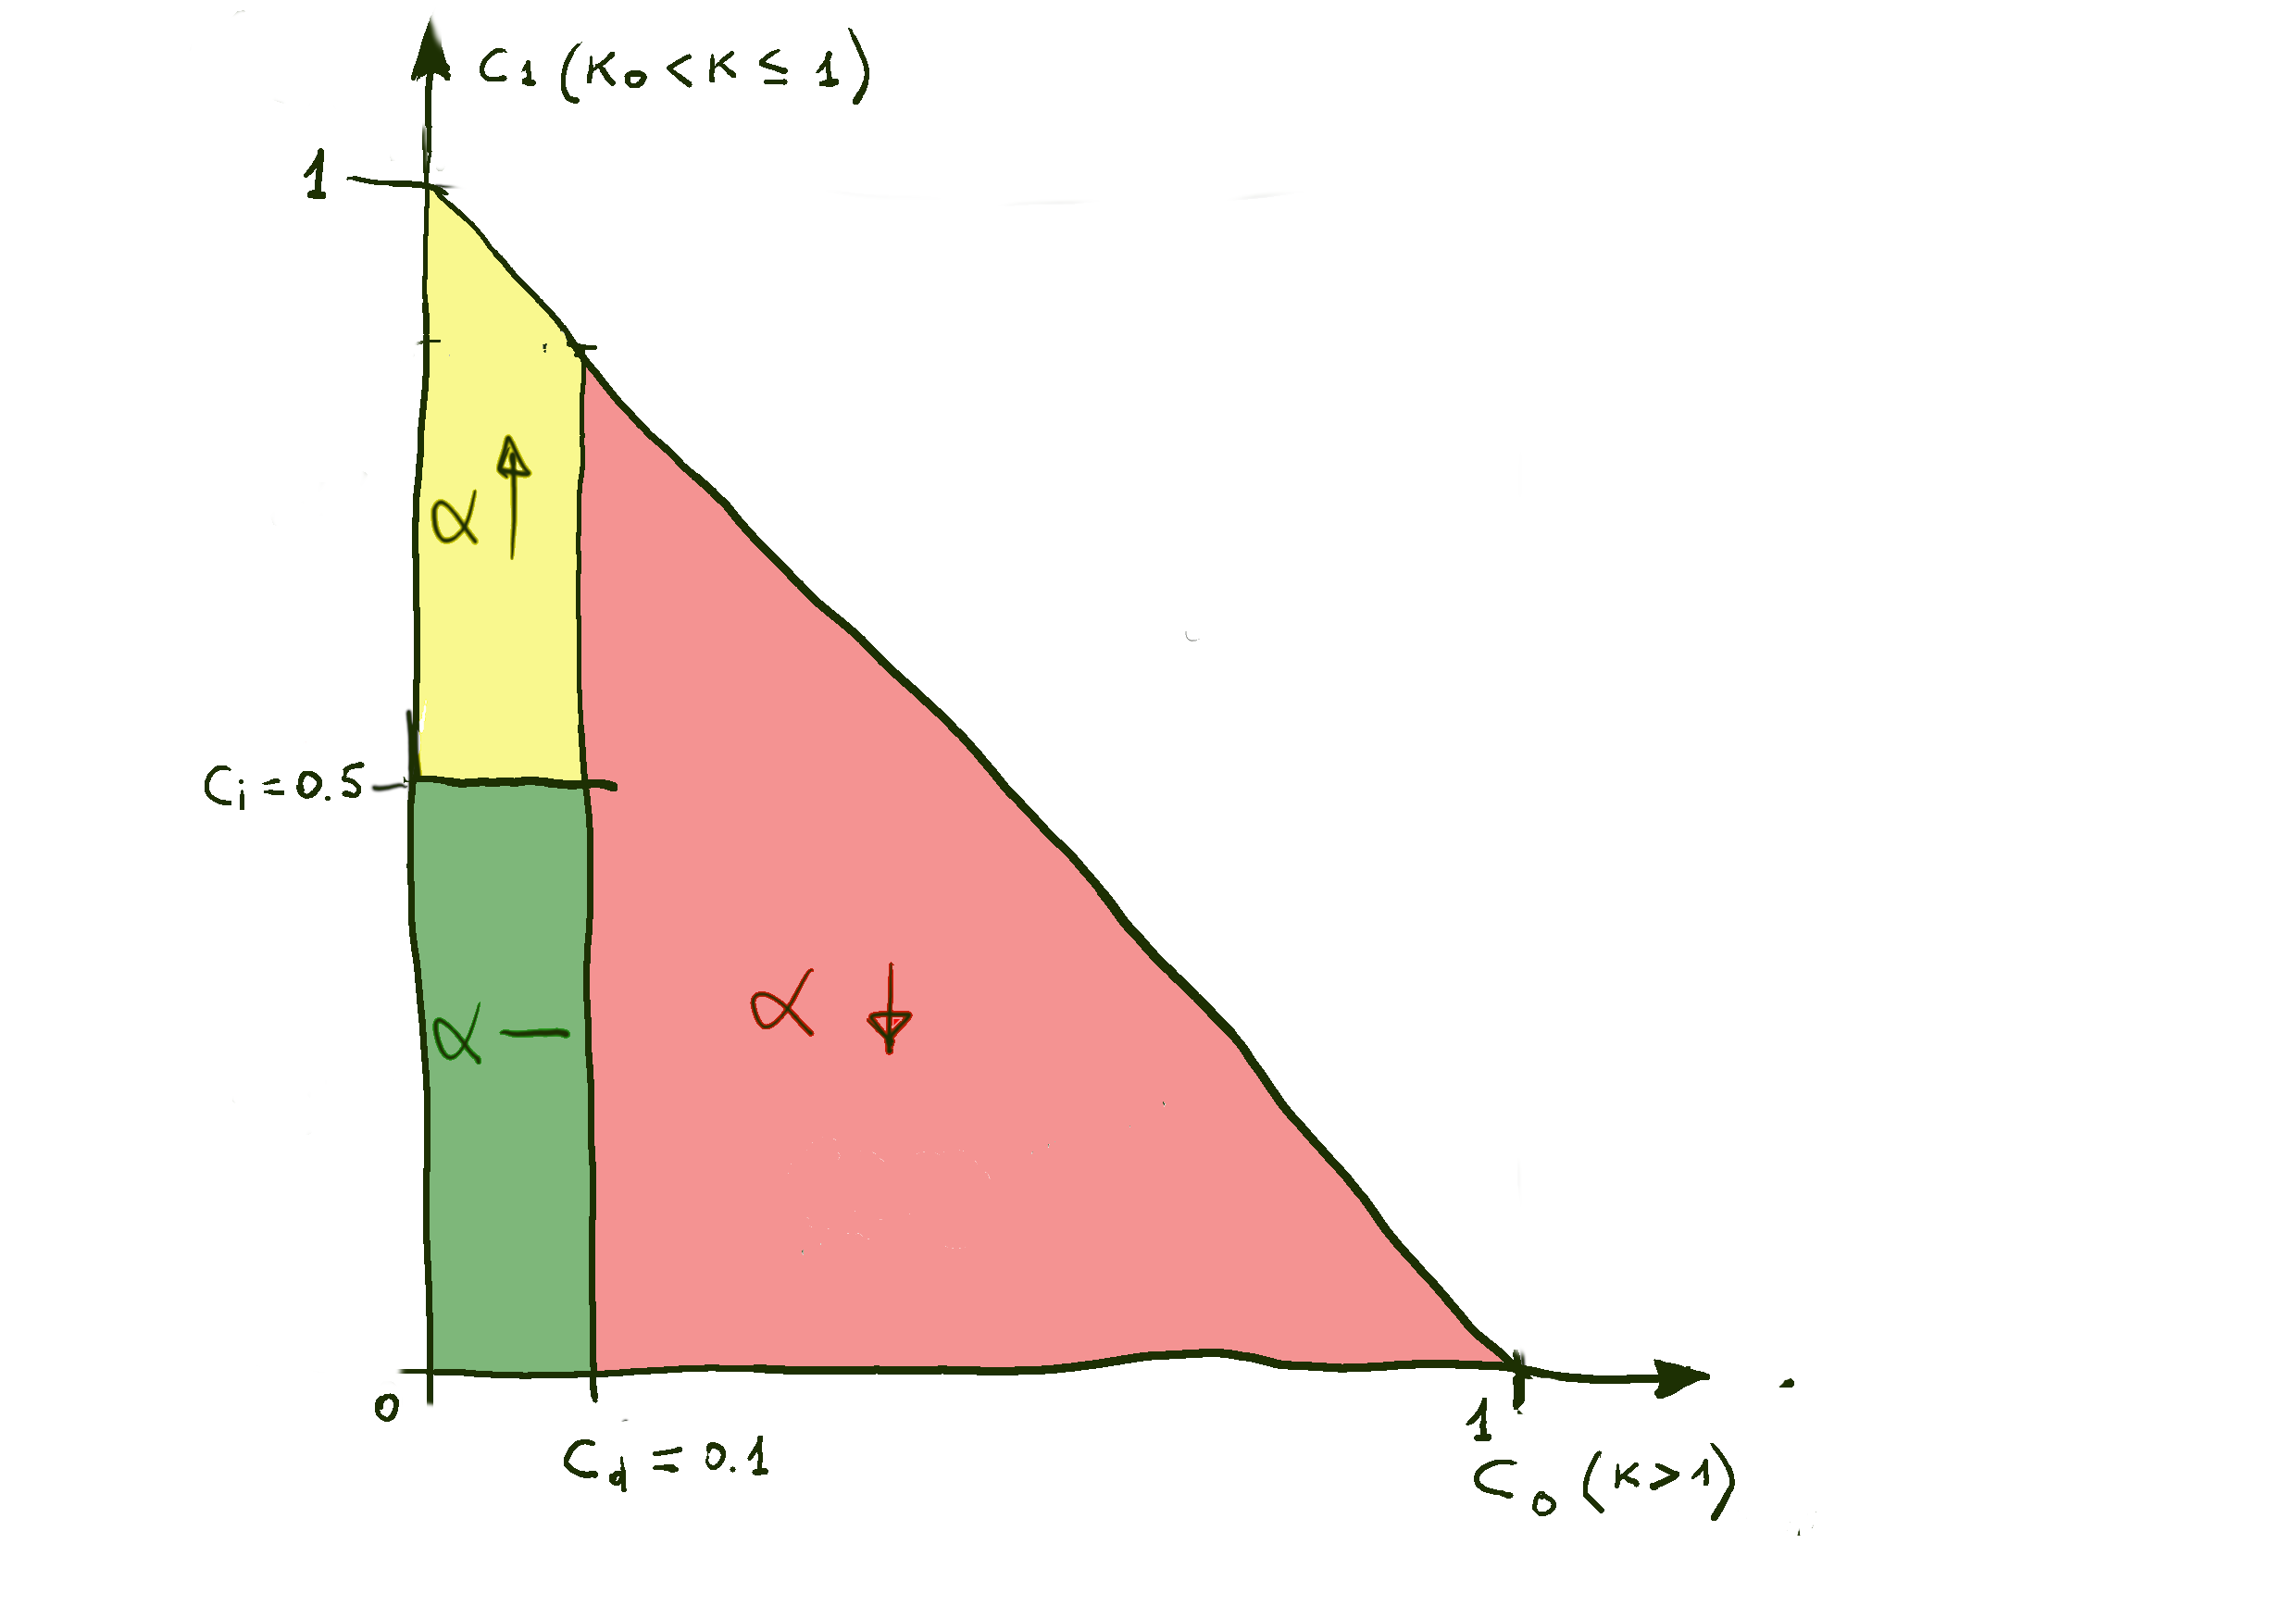
\includegraphics[width=\linewidth]{ann.png}
	\caption{Step classification}
	\label{fig:steps}
\end{figure}

\subsection{Policy Actor Indicators}

The actor computes the updated preferernces of current state by adding a step-size parameter to gradient and TD error

\begin{align*}
	h_{a, i}^*(s_t)&	= h_{a, i}(s_t) + \alpha_{h, i} \delta_{h_a, i}(t)
\end{align*}

To avoid computation overflow the preferences are constratints to a limited range e.g. $ (-7, +7) $.
The changes of preferences should also be limited to a fraction of the range $ (-\varepsilon_h, \varepsilon_h) $, so we can measure the squared distance of changes of preferences:
\begin{align}
\begin{split}
	J_{h,i}(t)&		= \alpha_{h, i}^2 \sum_a \delta_{h_a, i}^2(t)
\end{split}
\end{align}

A $ J_{h,i}(t) \ge \varepsilon_h^2 $ means a $ \alpha_{h,i} $ parameter value too high and $ J_{h,i}(t) \ll \varepsilon_h^2 $ means a $ \alpha_{h_i} $ parameter value too small, producing an uneffective changes on preferences.

Asserting we want to have a $ p $ fraction of samples with a $ J_{h,i}(t) < \varepsilon_h^2 $, we calculate $ J_{h, i, p} $ the $ p $ centile of $ J_{h, i}(t) $ and comupute the $ \gamma_{h,i} $ scale parameter
\begin{align}
\begin{split}
	\varepsilon_h^2&	= \gamma_{h,i}^2 J_{h,i,p}
	\\
	\gamma_{h,i}&			= \frac{\varepsilon_h}{\sqrt{J_{h,i}(t)}}
\end{split}
\end{align}

\subsection{Gaussian Policy Actor Indicators}

The actor computes the updated parameters of current state by adding a step-size parameter to gradient and TD error
\begin{align*}
	\delta_\mu&		= \frac{2}{\sigma^2}(a - \mu) \delta
	\\
	\delta_{h_\sigma}&	= \left[
		2\frac{(a - \mu)^2}{\sigma^2} - 1
	\right] \delta
\end{align*}

The updated gaussian parameters are
\begin{align*}
	\mu^*(s_t)&		= \mu(s_t) + \alpha_\mu \delta_\mu(s_t)
	\\
	h_\sigma^*(s_t)&	= h_\sigma(s_t) + \alpha_{h_\sigma}\delta_{h_\sigma}(s_t)
\end{align*}

We may consider the changes to the gaussian policy parameter limited to a defined range
\begin{align*}
	J_\mu(s_t)&								< \varepsilon^2_\mu
	\\
	|\mu^*(s_t) - \mu(s_t)|&				< \varepsilon_\mu
	\\
	|\delta_\mu(s_t)|&						< \varepsilon_\mu
	\\
	J_{h_\sigma}(s_t)&						< \varepsilon^2_{h_\sigma}
	\\
	[h_\sigma^*(s_t) - h_\sigma(s_t)]^2&	< \varepsilon^2_{h_\sigma}
	\\
	|\delta_{h_\sigma}(s_t)|&				< \varepsilon_{h_\sigma}
\end{align*}

An indicator $ J_\mu(s_t) \ge \varepsilon_\mu^2 $ means an $ \alpha_\mu $ parameter value too high, on the other hand an indicator$ J_\mu(s_t) \ll \varepsilon_\mu^2 $ means an $ \alpha_\mu $ parameter value too small.
An indicator $ J_{h_\sigma}(s_t) \ge \varepsilon_{h_\sigma}^2 $ means an $ \alpha_\sigma $ parameter value too high and an indicator $ J_{h_\sigma}(s_t) \ll \varepsilon_{h_\sigma}^2 $ means an $ \alpha_{h_\sigma} $ parameter value too small.

Asserting we want to have a $ p $ fraction of samples with a $ J_\mu(s_t) < \varepsilon_\mu^2 $, we calculate $ J_{\mu, p} $ the $ p $ centile of $ J_\mu(s_t) $ and comupute the $ \gamma_\mu $
\begin{align*}
	\varepsilon^2_\mu&	= \gamma_\mu^2 \sigma^2_\mu
	\\
	&					= \gamma^2_\mu J_\mu(s_t)
\end{align*}
\begin{align}
	\gamma_\mu&		= \frac{\varepsilon_\mu}{\sqrt{J_{\mu,p}}}
\end{align}

In the same way we have 
\begin{align}
	\gamma_{h_\sigma}&	= \frac{\varepsilon_{h\sigma}}{\sqrt{J_{h_\sigma, p} } }
\end{align}

\end{document}
